% \begin{frame}\frametitle{Testing on a ``toy'' sample}
% { \small
A set of 500\,000 $(a,b)$ events, Monte-Carlo generated according to the function
\(1 + x_1a + x_2a^2 + x_3b + x_4b^2\)
with parameters
\{$x_1 = 0.5$, $x_2 = 0.3$, $x_3 = 0.8$, $x_4 = 0.1$\};
and fitted using an event-by-event log.\ likelihood method with constraints
\(x_1^2 + x_1x_4 - x_4^2 = 0.29\), \(x_2^2/x_3 = 0.1125\).
% }

% Results:
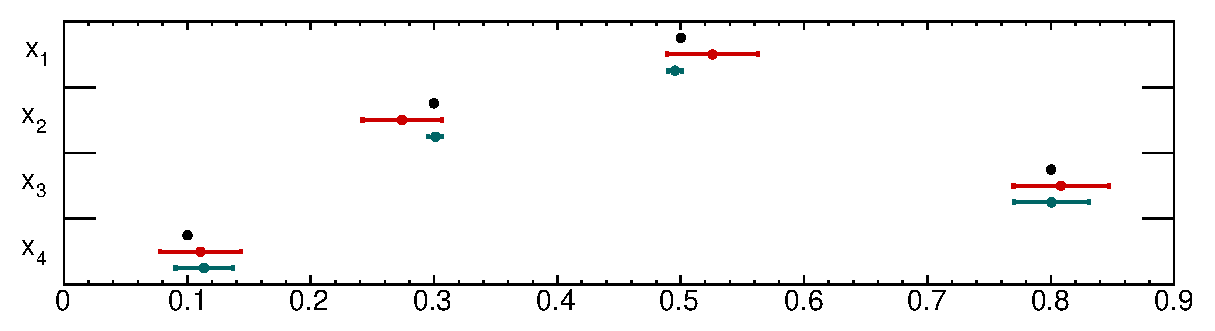
\includegraphics[width=1\textwidth]{pics/drawToy.eps}

\begin{tabular*}{1\textwidth}{@{\extracolsep{\fill}}cccc}\hline\hline
Parameter & True values & Unconstrained fit & Constrained fit \\\hline
$x_1$ & $0.5$ & $0.526 \pm 0.037$ & $0.496 \pm 0.006$ \\
$x_2$ & $0.3$ & $0.274 \pm 0.032$ & $0.301 \pm 0.006$ \\
$x_3$ & $0.8$ & $0.808 \pm 0.039$ & $0.801 \pm 0.030$ \\
$x_4$ & $0.1$ & $0.111 \pm 0.033$ & $0.114 \pm 0.023$ \\\hline\hline
\end{tabular*}
